\section{Introduction}

\subsection{UNISIM}

UNISIM provides several virtual platforms and a framework to ease the development of new virtual platforms.
A virtual platform is a software tool, often called simulator, that mimics the behavior of an electronic system so that software can run on it before silicon or FPGA implementation of that electronic system is available.
The simulated electronic system can include lots of microprocessors and devices.
Depending on the needed representativeness and simulator development budget, a simulator can be as simple as an instruction set simulator as well as a full system simulator.
A full system simulator, not only executes the microprocessor instruction set, like an instruction set simulator, but also simulates buses, I/O devices, sensors, actuators, so that real application workloads and operating systems can run on them.
Most of UNISIM virtual platforms are full system simulators, which means that they are sufficiently representative of the real hardware that whole operating systems (e.g. Linux, VxWorks), unmodified software stacks (e.g. an AUTOSAR software stack), and industrial applications can run on them.
The UNISIM virtual platforms are modular: a simulator is the assembly of properly configured simulation components (e.g. CPU, RAM, buses).
They are written in C/C++ and based on industry standards, like IEEE1666$^{TM}$, Accellera SystemC$^{TM}$ and Accellera SystemC$^{TM}$ TLM 2.0.

\noindent Some use cases of UNISIM virtual platforms are:
\begin{itemize}
\item Development of SystemC IPs (intellectual property) and new virtual platforms: UNISIM is an open development environment that comprise a SystemC module library, and a set of services (debugging, program loaders, …). It can be a fundation for the development of new SystemC IPs and new virtual virtual platforms.
\item Hybrid virtual platform: UNISIM/SystemC and an FPGA accelerator can be mixed to build some hybrid virtual platforms: for instance simulating processor cores within UNISIM/SystemC, and prototyping specialized IPs/devices within an FPGA accelerator. Hybridization allows using indifferently both UNISIM/SystemC IPs (on a standard host machine) and VHDL IPs (on an FPGA accelerator), but also speeding up simulation of large systems.
\item Non-intrusive debugging and testing of software: It means that, unlike on the real hardware, software can be debugged and tested without affecting either its functional and/or temporal behavior.
With such virtual instrumentation, the user can seamlessly stop and resume execution of software, profile the software, inspect the system status, inject values on the sensors, modify the state of program variables and microprocessor/device registers, and then analyze the result without modifying the software.
\item Hardware/software integration: software stack can be debugged and tested within a representative hardware environment before the availability of either the FPGA prototypes or the real hardware.
The software stack can be composed of low level software (e.g. drivers), of a real-time operating system, and of applications generated from high level models (Papyrus, Matlab Simulink, Statemate Stateflow, …)
\end{itemize}

Several open source virtual platforms for different targets (ARM, PowerPC, Star12X, and TMS320C3X) and different hosts (Linux, Windows, Mac OS X) are available for download here.
These virtual platforms have been evaluated and used in various industry domains such as automotive, avionic, military, electrical equipments for medium tension, nuclear safety.

\subsection{Virtex 5 FXT Simulator}

\begin{figure}[p]
	\begin{center}
		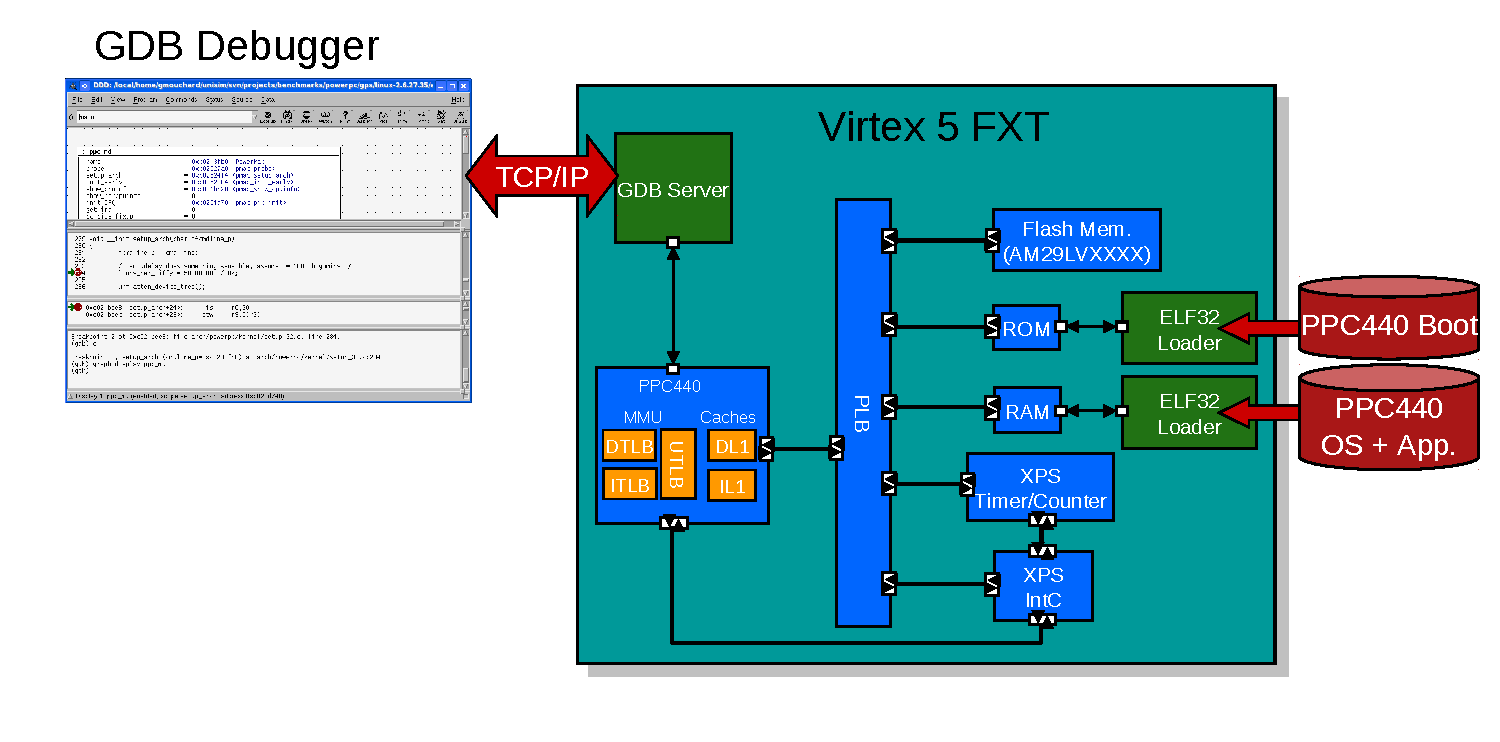
\includegraphics[width=\textwidth]{virtex5fxt/fig_schematic.pdf}
	\end{center}
	\caption{UNISIM Virtex 5 FXT simulator schematic.}
	\label{fig:simulator_schematic}
\end{figure}

\begin{table}[p]
	\begin{center}
		\begin{tabular}{|l|l|l|}
		\hline
		\multicolumn{1}{|c|}{\textbf{Address range}} & \multicolumn{1}{|c|}{\textbf{Component name}} & \multicolumn{1}{|c|}{\textbf{Hardware device}}\\
		\hline
		\texttt{0x00000000-0x0003ffff} & \texttt{ram} & 256 MB RAM\\
		\hline
		\texttt{0x81400000-0x8140ffff} & \texttt{gpio-leds-8bit} & XPS GPIO\\
		\hline
		\texttt{0x81420000-0x8142ffff} & \texttt{gpio-5-leds-positions} & XPS GPIO\\
		\hline
		\texttt{0x81440000-0x8144ffff} & \texttt{gpio-push-buttons-5bit} & XPS GPIO\\
		\hline
		\texttt{0x81460000-0x8146ffff} & \texttt{gpio-dip-switches-8bit} & XPS GPIO\\
		\hline
		\texttt{0x81800000-0x8180ffff} & \texttt{intc} & XPS IntC\\
		\hline
		\texttt{0x83c00000-0x83c0ffff} & \texttt{timer} & XPS Timer/Counter\\
		\hline
		\texttt{0x84000000-0x8400ffff} & \texttt{uart-lite} & XPS UART Lite\\
		\hline
		\texttt{0xfc000000-0xfdffffff} & \texttt{flash} & S29GL256P\\
		\hline
		\texttt{0xfffc0000-0xffffffff} & \texttt{bram} & 256 KB BRAM\\
		\hline
		\end{tabular}
	\end{center}
	\caption{Simulator memory mapping.}
	\label{table:memory_mapping}
\end{table}

The UNISIM Virtex 5 FXT is a virtual platform that tries to mimic a Xilinx ML507 development board that include a Xilinx Virtex 5 FXT (FPGA + PPC440).

\noindent The UNISIM Virtex 5 FXT simulator, which Figure~\ref{fig:simulator_schematic} shows the schematic, implements the following:
\begin{itemize}
	\item PPC440 Embedded Processor Block (UG200~\cite{UG200}):
		\begin{itemize}
			\item All the PPC440x5 \cite{PPC440x5} instruction set of a Xilinx Virtex 5 FXT
			\item Optional FPU that is similar to Xilinx FPU APU \cite{APU_FPU}
			\item PowerPC Book E MMU (shadow ITLB, shadow DTLB, unified TLB)
			\item Caches (instruction and data)
			\item Integrated timers (decrementer, fixed interval, watchdog)
			\item Exception handling mechanisms
			\item DCR (device control register) bus controller
			\item Crossbar
			\item MCI (Memory Controller Interface)
			\item MPLB (master processor local bus) interface
			\item SPLB0 and SPLB1 (slave processor local bus) interfaces
		\end{itemize}
	\item MPLB (master processor local bus) link
	\item 256 MB RAM on MCI
	\item 256 KB BRAM on MPLB
	\item XPS IntC interrupt controller (v2.01a) \cite{XPS_INTC} on MPLB
	\item XPS Timer/Counter (v1.02a) \cite{XPS_TIMER_COUNTER} on MPLB
	\item Spansion 256 Mbits (32 MB) S29GL256P off-chip flash memory \cite{S29GLP} on MPLB
	\item XPS UART Lite (v1.01a) \cite{XPS_UART_LITE} on MPLB
	\item Four XPS GPIO modules (v2.00a) \cite{XPS_GPIO} on MPLB connected to two LED boards and two DIP switch/push buttons boards
\end{itemize}

\noindent Several stub modules are currently integrated in the simulator to test the XPS Timer/Counter module:
\begin{itemize}
\item GenerateOut stubs connected on XPS Timer/Counter « GenerateOut » outputs
\item PWM stub connected on XPS Timer/Counter « PWM0 » output
\item CaptureTrigger stubs (optional randomized outputs) connected on XPS Timer/Counter « CaptureTrigger » inputs
\item SPLB stubs
\item DCR stubs
\end{itemize}

\cleardoublepage

\noindent The simulator also supports the following features :
\begin{itemize}
\item Loading of ELF32, ELF64 \cite{ELF} and Motorola S19 (S-Record) \cite{S19} files
\item An integrated console debugger that supports debugging both at assembly level and source level (e.g. C source code). Source level debugging is only available for ELF binary files including DWARF v2 or v3 \cite{DWARF3} debugging informations
\item Support for the GDB \cite{GDB} serial remote protocol over TCP/IP. That allows debugging a binary running into the simulator at assembly and/or source level using the GNU debugger (aka GDB)
\item Support for a telnet console over the XPS UART Lite
\end{itemize}

Table~\ref{table:memory_mapping} shows the simulator memory mapping.

\noindent The 1.0 release of the simulator is composed of:
\begin{itemize}
\item the simulator source code: unisim-virtex5fxt-1.0beta10.tar.gz
\item the present documentation
\end{itemize}

Please follow the installation instructions in Section~\ref{building_simulator} to get the simulator building on your own building environment.
Section~\ref{getting_started} presents the basics for using the simulator.
Section~\ref{examples_of_use} presents some examples of use of the simulator.
Appendix~\ref{techref} contains the technical references (generated) of the simulator.

\section{Building the simulator}
\label{building_simulator}

\subsection{Requirements}

\noindent The following tools or libraries must be installed:
\begin{itemize}
\item GNU C++ compiler (aka. g++)
\item GNU Flex (aka. flex)
\item GNU Bison (aka. bison)
\item Standard GNU C++ library (aka. libstdc++-dev that comes with g++)
\item Boost (aka. libboost-dev)
\item Editline/Libedit (aka. libedit-dev)
\item zlib (aka. zlib1g-dev)
\item libxml2 (aka. libxml2-dev)
\end{itemize}

\subsection{Installing SystemC 2.3}
\subsubsection{Download the source code}
Register at \url{http://www.accellera.org} and then download systemc-2.3.0.tgz from the Accelera SystemC standards download page.

\subsubsection{Uncompressing the source code tarballs}
\begin{script}
   $ tar zxvf systemc-2.3.0.tgz
\end{script}
  
This will uncompress the source of SystemC in directory systemc-2.3.0. 

\subsubsection{Configuring SystemC}
To handle threads, SystemC relies on QuickThreads, a fast implementation of user's threads. QuickThreads speeds-up threads switching compared to the slower kernel POSIX threads and thus considerably improves overall simulation performance. To configure the SystemC building process with the built-in QuickThreads (recommended), do the following at the command prompt:
\begin{script}
   $ cd systemc-2.3.0
   $ mkdir objdir
   $ cd objdir
   $ mkdir ${HOME}/systemc
   $ ../configure --prefix=${HOME}/systemc --disable-shared
\end{script}
However, if you intend to instrument your simulator (e.g. with valgrind) to debug the simulator memory leaks, bad memory accesses, pointers, and uninitialized memory reads, you should use the slower kernel POSIX threads. To configure the SystemC building process with the kernel POSIX threads, do the following at the command prompt:
\begin{script}
   $ cd systemc-2.3.0
   $ mkdir objdir
   $ cd objdir
   $ mkdir ${HOME}/systemc
   $ ../configure --prefix=${HOME}/systemc --enable-pthreads --disable-shared
\end{script}

\subsubsection{Compiling and installing SystemC}
To compile SystemC, do the following at the command prompt:
\begin{script}
   $ make
   $ make install
\end{script}

\subsection{Building the UNISIM Virtex 5 FXT simulator}
\subsubsection{Uncompressing the source code tarball}
\begin{script}
   $ tar zxvf unisim-virtex5fxt-1.0beta10.tar.gz
\end{script}

\subsubsection{Configuring the simulator building process}
\begin{script}
  $ cd unisim-virtex5fxt-1.0beta10
  $ ./configure \
          --with-systemc=${HOME}/systemc
\end{script}

\subsubsection{Compiling the simulator}
\begin{script}
   $ make
\end{script}

\noindent The simulator binaries are in \texttt{virtex5fxt/bin} subdirectory.
The simulators comes in four flavors in:
\begin{itemize}
\item \texttt{unisim-virtex5fxt-1.0beta10}: release simulator without FPU
\item \texttt{unisim-virtex5fxt-wfpu-1.0beta10}: release simulator with FPU
\item \texttt{unisim-virtex5fxt-debug-1.0beta10}: developement simulator
\item \texttt{unisim-virtex5fxt-wfpu-debug-1.0beta10}: developement simulator with FPU
\end{itemize}

\section{Cross-compiling the simulator}

This section explains how to build (i.e. cross-compile) the simulator for a host system type (e.g. Windows) from another build system type (e.g. Linux/i386).
The simulator is built on the build machine whereas it will run on the host machine.
In later sub-sections, we consider cross-compiling the simulator for Windows from a Linux distribution using the mingw32 GCC cross-compiler.
Most Linux distributions provide a mingw32 tool chain as a set of packages.
Once installed the mingw32 tool chain binary file names are prefixed with:
\begin{itemize}
\item \texttt{i586-mingw32msvc-} on Ubuntu and Debian Linux distributions
\item \texttt{i686-pc-mingw32-} on RedHat, Fedora, and SUSE Linux distributions
\item \texttt{i586-pc-mingw32-} on Mandriva and Mageia Linux distributions
\end{itemize}
The later sub-sections will refer to the mingw32 tool chain of Ubuntu and Debian Linux distributions.

\subsection{Requirements}

\noindent The following tools must be installed on the Linux build system:
\begin{itemize}
\item GNU C++ cross-compiler for the host system type (aka. i586-mingw32msvc-g++)
\item GNU Flex (aka. flex)
\item GNU Bison (aka. bison)
\item Standard GNU C++ library for the host machine (aka. libstdc++)
\end{itemize}

\subsection{Installing a cross-compiled SystemC 2.3.0}
\subsubsection{Download the source code}
Register at \url{http://www.accellera.org} and then download systemc-2.3.0.tgz from the Accellera SystemC standards download page.

\subsubsection{Uncompressing the source code tarballs}
\begin{script}
   $ tar zxvf systemc-2.3.0.tgz
\end{script}
  
This will uncompress the source of SystemC in directory systemc-2.3.0. 

\subsubsection{Configuring SystemC}
To configure, cross-compile, and install SystemC in your home directory, do the following at the command prompt: 

\begin{script}
   $ cd systemc-2.3.0
   $ mkdir objdir
   $ cd objdir
   $ mkdir ${HOME}/systemc-mingw32
   $ ../configure --prefix=${HOME}/systemc-mingw32 --host=i586-mingw32msvc --disable-shared
\end{script}

\subsubsection{Cross-compiling and installing SystemC}
To cross-compile SystemC, do the following at the command prompt: 
\begin{script}
   $ make
   $ make install
\end{script}

\subsection{Cross-compiling zlib}

Download the source code tarball at \url{http://zlib.net/zlib-1.2.5.tar.gz}.
Uncompress the source code tarball and cross-compile the library:
\begin{script}
   $ tar zxvf zlib-1.2.5.tar.gz
   $ cd zlib-1.2.5
   $ mkdir ${HOME}/zlib-mingw32
   $ make -f win32/Makefile.gcc \
     PREFIX=i586-mingw32msvc- \
     BINARY_PATH=${HOME}/zlib-mingw32/bin \
     INCLUDE_PATH=${HOME}/zlib-mingw32/include \
     LIBRARY_PATH=${HOME}/zlib-mingw32/lib \
     SHARED_MODE=1 install
   $ mv ${HOME}/zlib-mingw32/bin/zdll.a ${HOME}/zlib-mingw32/bin/z.dll.a
\end{script}

\subsection{Cross-compiling libxml2}

Download the source code tarball at \url{ftp://xmlsoft.org/libxml2/libxml2-2.7.8.tar.gz}.
Uncompress the source code tarball and cross-compile the library:
\begin{script}
   $ tar zxvf libxml2-2.7.8.tar.gz
   $ cd libxml2-2.7.8
   $ mkdir ${HOME}/libxml2-mingw32
   $ ./configure  --host=i586-mingw32msvc \
         --without-python --with-zlib=${HOME}/zlib-mingw32 \
          CPPFLAGS='-DLIBXML_STATIC'
   $ make
   $ make install prefix=${HOME}/libxml2-mingw32
\end{script}

\subsection{Cross-compiling Boost}

Download the source code tarball at \url{http://downloads.sourceforge.net/boost/boost\_1\_47\_0.tar.bz2}.
Uncompress the source code tarball and cross-compile the library:

\begin{script}
   $ tar jxvf boost_1_47_0.tar.bz2
   $ cd boost_1_47_0
   $ mkdir ${HOME}/boost-mingw32
   $ ./bootstrap.sh --without-icu
   $ MINGW32_VERSION=$(i586-mingw32msvc-g++ -v 2>&1 | tail -1 | awk '{print $3}' | cut -f 1 -d '-')
   $ echo "using gcc : ${MINGW32_VERSION} :
                 i586-mingw32msvc-g++ :
                 <rc>i586-mingw32msvc-windres
                 <archiver>i586-mingw32msvc-ar
            ;" > user-config.jam
   $ ./bjam toolset=gcc target-os=windows variant=release threading=multi threadapi=win32 \
          link=shared runtime-link=shared --prefix=${HOME}/boost-mingw32 --user-config=user-config.jam \
          --without-mpi --without-python -sNO_BZIP2=1 -sZLIB_BINARY=z.dll \
          -sZLIB_INCLUDE=${HOME}/zlib-mingw32/include -sZLIB_LIBPATH=${HOME}/zlib-mingw32/lib \
          --layout=tagged install
\end{script}

\subsection{Cross-compiling the UNISIM Virtex 5 FXT simulator}
\subsubsection{Uncompressing the source code tarball}
\begin{script}
   $ tar zxvf unisim-virtex5fxt-1.0beta10.tar.gz
\end{script}

\subsubsection{Configuring the simulator building process}
\begin{script}
  $ cd unisim-virtex5fxt-1.0beta10
  $ ./configure.cross \
          --host=i586-mingw32msvc \
          --with-systemc=${HOME}/systemc-mingw32 \
          --with-zlib=${HOME}/zlib-mingw32 \
          --with-libxml2=${HOME}/libxml2-mingw32 \
          --with-boost=${HOME}/boost-mingw32 \
          CXXFLAGS='-O3 -g3 -Wall'
\end{script}

\subsubsection{Cross-compiling the simulator}
\begin{script}
   $ make -f Makefile.cross
\end{script}

\noindent The simulator binaries are in \texttt{virtex5fxt/bin} subdirectory.
The simulators comes in four flavors in:
\begin{itemize}
\item \texttt{unisim-virtex5fxt-1.0beta10.exe}: release simulator without FPU
\item \texttt{unisim-virtex5fxt-wfpu-1.0beta10.exe}: release simulator with FPU
\item \texttt{unisim-virtex5fxt-debug-1.0beta10.exe}: developement simulator
\item \texttt{unisim-virtex5fxt-wfpu-debug-1.0beta10.exe}: developement simulator with FPU
\end{itemize}

The simulator binaries may need some DLLs from mingw32 (e.g. \texttt{libgcc\_s*.dll}) or third party libraries (e.g. \texttt{libxml2-2.dll}).
Place these DLLs in the \texttt{virtex5fxt/bin} subdirectory.
If you prefer not to use DLLs, add \texttt{LDFLAGS=-static} to the \texttt{configure.cross} command line arguments.
The simulator binaries can run natively run on a Windows host system, or an emulated Windows using \texttt{wine} windows emulator.

\section{Getting started}
\label{getting_started}

In this section, we present the basics for using the simulator.
More details are available in Appendix~\ref{techref}.

\subsection{Run-time configuration}

The simulator has a parametrization system that allows configuring individual simulator components, that is the hardware components, and the services.
\noindent The simulator stores its configuration (a set of parameters) in a XML configuration file. 
\newline\\
\noindent The simulator can provide the user with a default XML configuration file with option \texttt{-g}:
\begin{script}
   $ unisim-virtex5fxt-wfpu-1.0beta10 -g default_sim_config.xml
\end{script}

The XML configuration file can be edited, and then reloaded by the simulator with option \texttt{-c}:
\begin{script}
   $ unisim-virtex5fxt-wfpu-1.0beta10 -c sim_config.xml
\end{script}

\noindent The user can also simply set the value of an individual parameter with option \texttt{-s}:
\begin{script}
   $ unisim-virtex5fxt-wfpu-1.0beta10 -s enable-inline-debugger=true
\end{script}

\noindent The simulator can prints the list of parameter set on the console with option \texttt{-l}:
\begin{script}
   $ unisim-virtex5fxt-wfpu-1.0beta10 -l
\end{script}

\noindent In general, each simulator components have log messages that can be switched on or off using a parameter named \texttt{verbose} (or approching):
\begin{script}
   $ unisim-virtex5fxt-wfpu-1.0beta10 -s cpu.verbose-exception=true
\end{script}

\noindent The simulator accepts any combination of the above options.
For example, you can combine these options to change the value of one or more parameters in an XML configuration file:
\begin{script}
   $ unisim-virtex5fxt-wfpu-1.0beta10 -c sim_config.xml -s enable-inline-debugger=true -g sim_config.xml
\end{script}

\subsection{Loading binaries}
\label{loading_binaries}

The simulators has a multi-format loader service that can detect the format of binaries and accordingly instantiate the right loader.
The user can set the list of binary files to load in Parameter loader.filename, each filenames being separated by a comma:
\begin{script}
   $ unisim-virtex5fxt-wfpu-1.0beta10 -s loader.filename='boot.elf,vmlinux,device_tree.dtb,initrd.img'
\end{script}
In the hypothetic case where the multi-format loader would wrongly guess the format of a binary, the user tells the loader what is the format of the binary file:
\begin{script}
   $ unisim-virtex5fxt-wfpu-1.0beta10 \
     -s loader.filename='boot.elf:elf32,vmlinux:elf32,device_tree.dtb:raw,initrd.img:raw'
\end{script}

\noindent If, for any reason (virtual memory, self relocation), the simulator must load a binary file to an address that is not the final address indicated in the binary file itself, the user tells the loader to override (when possible) the base address:
\begin{script}
   $ unisim-virtex5fxt-wfpu-1.0beta10 \
        -s loader.filename='boot.elf,vmlinux,device_tree.dtb,initrd.img' \
        -s loader.file1.base-addr=0 \
        -s loader.file1.force-base-addr=true
\end{script}

\subsection{Serial console}

The simulator comes with a UART Lite module on MPLB that the target application can use as a serial console.
The simulator telnet service, that is actually a server for the telnet protocol, manages communication between the real network and the virtual UART Lite module.
The combination of the UART Lite module, the telnet service and a serial console aware target application, enables using a real telnet client (running on the host machine or any machine on the internet) as virtual serial console.

To enable the serial console, do the following at the command prompt:
\begin{script}
   $ unisim-virtex5fxt-wfpu-1.0beta10 \
        -s enable-telnet=true \
        -s telnet.telnet-tcp-port=1234
\end{script}

During initialization, the simulator waits for a telnet client connection on the telnet port.
In another console, connect a telnet client to the simulator:
\begin{script}
   $ telnet localhost 1234
\end{script}

At this point, the user can interact with the target application using the telnet client.

\subsection{Using the builtin debugger}

The simulator has an integrated debugger for debugging the target application an a non-intrusive manner.

To enable the inline-debugger, do the following at the command prompt:
\begin{script}
   $ unisim-virtex5fxt-wfpu-1.0beta10 -s enable-inline-debugger=true
\end{script}

The user can enter classical debug commands from the debugger, such as putting breakpoints, watchpoints, stepping instructions, disassembling, dumping memory regions, etc.

To obtain help within the debugger, uses the debugger command \texttt{help}:
\begin{script}
   inline-debugger> help
\end{script}

\subsection{Using a GNU crosstool chain}

\subsubsection{Building a GNU crosstool chain}
\label{building_crosstool_chain}

A crosstool chain is a tool chain to create and manipulate binary programs for a target architecture and operating system (e.g. PowerPC/Linux) that are different from host architecture and operating system (e.g. x86/Linux) that runs the tool chain.
Building a GNU crosstool chain from scratch is a very tedious task.
The process consists of a quite high number of undocumented steps, and mostly relies on the users experience.
Fortunately a community sharing its experience, the crossgcc mailing list, actively supports a tool, crosstool-NG, that considerably simplifies the process of building a crosstool chain.
Xilinx Virtex-5 FXT embedded processor is a PPC440x5 and Xilinx Platform Studio provides a PowerPC hardware FPU.
Hence, from now, we will focus our effort on creating a crosstool chain with GNU GCC 4.7.2 (\texttt{gcc} and \texttt{g++}), GNU C library 2.16.0 (\texttt{glibc}), GNU binutils 2.22 (\texttt{ld}, \texttt{objdump}, and \texttt{readelf}), and GNU GDB 7.4.1 (\texttt{gdb}) for target \texttt{powerpc-440fp-linux-gnu}.

\begin{enumerate}
\item Get crosstool-NG: Download the crosstool-NG archive (e.g crosstool-ng-1.18.0.tar.bz2) from this page: \url{http://crosstool-ng.org}
\item Uncompress crosstool-NG archive:
\begin{script}
   $ tar jxvf crosstool-ng-1.18.0.tar.bz2
\end{script}
\item Configure crosstool-NG build:
\begin{script}
   $ cd crosstool-ng-1.18.0
   $ ./configure --enable-local
\end{script}  
\item Compile crosstool-NG
\begin{script}
   $ make
\end{script}
\item Configure the crosstool chain build as shown on Figure~\ref{fig:ctng_configuration}:
\begin{script}
   $ ./ct-ng menuconfig
\end{script}
\item Build the crosstool chain (this may take tens of minutes/hours):
\begin{script}
   $ ./ct-ng build
\end{script}
\item You crosstool chain is ready in \texttt{\$\{HOME\}/crosstool/powerpc-440fp-linux-gnu}
\end{enumerate}

\begin{figure}[p]
\begin{center}
\begin{script}
Paths and misc options  --->
(${HOME}/crosstool/powerpc-440fp-linux-gnu) Prefix directory

Target options  --->
        Target Architecture (powerpc)  --->
    (440fp) Emit assembly for CPU
    (440fp) Tune for CPU
        Floating point: (hardware (FPU))  --->

Toolchain options  --->
    (440fp) Tuple's vendor string

Operating System  --->
    Target OS (linux)  --->
    Linux kernel version (3.7.3)  --->

Binary utilities  --->
    binutils version (2.22)  --->

C compiler  --->
    gcc version (4.7.2)  --->
    [*] C++
    [ ] Link libstdc++ statically into the gcc binary

C-library  --->
    C library (glibc)  --->
    glibc version (2.16.0)  --->
    (-g) gcc extra flags
    Minimum supported kernel version (Specific kernel version) --->
      Specific kernel version
    (2.6.9) Minimum kernel version to supports

Debug facilities  --->
    [*] gdb  --->

\end{script}
\end{center}
\caption{crosstool chain build configuration (changes from default only) for Crosstool-NG 1.18.0.}
\label{fig:ctng_configuration}
\end{figure}

\cleardoublepage

\subsubsection{Using cross-GCC}

A GCC cross-compiler together with a LD cross-linker can be used to create binaries for the target machine from the host machine:
\begin{script}
   $ ${HOME}/crosstool/powerpc-440fp-linux-gnu/bin/powerpc-440fp-linux-gnu-gcc \
                     nodefaultlibs -nostdlib -mcpu=440fp -c hello.c -o hello.o
   $ ${HOME}/crosstool/powerpc-440fp-linux-gnu/bin/powerpc-440fp-linux-gnu-ld hello.lds -o hello.elf
\end{script}

\noindent Simulator can directly loads such binary files, see Section~\ref{loading_binaries}.

\subsubsection{Using cross-GDB}

GNU GDB client can debug applications running on a remote/local host on the network.
The application is run under the control of program \texttt{gdbserver} while program \texttt{gdb} only manages interactions with the user.
Program \texttt{gdbserver} and \texttt{gdb} communicates over the TCP/IP network using a documented serial remote protocol.
The simulator has a GDB server service that implements the GDB serial remote protocol, so that the simulator can acts as Program \texttt{gdbserver} from the GDB client point of view.

To enable the simulator GDB server, do the following at the command prompt:
\begin{script}
   $ unisim-virtex5fxt-wfpu-1.0beta10 -s enable-gdb-server=true -s gdb-server.tcp-port=1234
\end{script}

During initialization, the simulator waits for a GDB client connection on the GDB server TCP/IP port.
In another console, connect a GDB client to the simulator:
\begin{script}
   $ powerpc-440fp-linux-gnu-gdb boot.elf
   (gdb) target remote :1234
\end{script}

\section{Examples of use}
\label{examples_of_use}

In this section, we present some examples of use for the simulator.
We provide you with scripts and makefiles to build in an automatic manner all the examples.
These examples are available for download in source and binary forms on our web site (\url{http://unisim-vp.org}):
\begin{itemize}
\item Basic system level unit tests: [\href{http://unisim-vp.org/site/downloads/virtual-platforms/powerpc/virtex5fxt/unisim-virtex5fxt-basic-system-level-unit-tests-bin-v3.tar.gz}{hyperlink to binaries}], [\href{http://unisim-vp.org/site/downloads/virtual-platforms/powerpc/virtex5fxt/unisim-virtex5fxt-basic-system-level-unit-tests-source-v3.tar.gz}{hyperlink to sources}]
\item MiBench version 1: [\href{http://unisim-vp.org/site/downloads/other/benchmarks/mibench/mibench-v1-bin-powerpc-440fp-linux-gnu-v3.tar.gz}{hyperlink to binaries}], [\href{http://unisim-vp.org/site/downloads/other/benchmarks/mibench/mibench-v1-source-v3.tar.gz}{hyperlink to sources}]
\item light weight Linux distribution: [\href{http://unisim-vp.org/site/downloads/other/benchmarks/linux-distro/unisim-virtex5fxt-linux-distro-bin-v3.tar.gz}{hyperlink to binaries}], [\href{http://unisim-vp.org/site/downloads/other/benchmarks/linux-distro/unisim-virtex5fxt-linux-distro-source-v3.tar.gz}{hyperlink to sources}]
\end{itemize}

To build the examples you need a functional cross tool-chain for Target \texttt{powerpc-440fp-linux-gnu}, see Section~\ref{building_crosstool_chain}.
In later sub-sections, we assume that your cross tool-chain is installed in \texttt{\$\{HOME\}/crosstool/powerpc-440fp-linux-gnu}

\subsection{Basic system level tests}

Table~\ref{table:basic_system_test_summary} shows a summary of basic system level tests.

\begin{table}[h]
	\begin{center}
		\small
		\begin{tabular}{|l|l|l|l|l|l|}
		\hline
		\multicolumn{1}{|c|}{\textbf{Test Name}} &
		\multicolumn{1}{|c|}{\textbf{Directory}} &
		\multicolumn{1}{|c|}{\VROT{\textbf{IntC}}} &
		\multicolumn{1}{|c|}{\VROT{\textbf{Timer}}} &
		\multicolumn{1}{|c|}{\VROT{\textbf{UART Lite}}} &
		\multicolumn{1}{|c|}{\VROT{\textbf{NOR Flash}}}\\
		\hline
		Echo &
		\texttt{\footnotesize xps\_uart\_lite/echo} &
		\X &
		   &
		\X &
		   \\
		\hline
		Poll &
		\texttt{\footnotesize xps\_timer/poll} &
		   &
		\X &
		\X &
		   \\
		\hline
		Gen &
		\texttt{\footnotesize xps\_timer/gen} &
		\X &
		\X &
		\X &
		   \\
		\hline
		Cap &
		\texttt{\footnotesize xps\_timer/cap} &
		\X &
		\X &
		\X &
		   \\
		\hline
		PWM &
		\texttt{\footnotesize xps\_timer/pwm} &
		\X &
		\X &
		\X &
		   \\
		\hline
		Autoselect &
		\texttt{\footnotesize s29gl256p/autoselect} &
		\X &
		   &
		\X &
		\X \\
		\hline
		CFI query &
		\texttt{\footnotesize s29gl256p/cfi\_query} &
		\X &
		   &
		\X &
		\X \\
		\hline
		Chip erase &
		\texttt{\footnotesize s29gl256p/chip\_erase} &
		\X &
		   &
		\X &
		\X \\
		\hline
		Sector erase &
		\texttt{\footnotesize s29gl256p/sector\_erase} &
		\X &
		   &
		\X &
		\X \\
		\hline
		Single word programming &
		\texttt{\footnotesize s29gl256p/single\_word\_programming} &
		\X &
		   &
		\X &
		\X \\
		\hline
		Unlock bypass chip erase &
		\texttt{\footnotesize s29gl256p/unlock\_bypass\_chip\_erase} &
		\X &
		   &
		\X &
		\X \\
		\hline
		Unlock bypass sector erase &
		\texttt{\footnotesize s29gl256p/unlock\_bypass\_sector\_erase} &
		\X &
		   &
		\X &
		\X \\
		\hline
		Unlock bypass word programming &
		\texttt{\footnotesize s29gl256p/unlock\_bypass\_word\_programming} &
		\X &
		   &
		\X &
		\X \\
		\hline
		Write buffer programming &
		\texttt{\footnotesize s29gl256p/write\_buffer\_programming} &
		\X &
		   &
		\X &
		\X \\
		\hline
		\end{tabular}
	\end{center}
	\caption{Summary of basic system level tests.}
	\label{table:basic_system_test_summary}
\end{table}

\subsubsection{Description}

\noindent \textbf{Echo}.The test reads characters from the serial console.
It prints the read characters on the serial console.

\noindent \textbf{Poll}. The test polls the timer/counter \#0.
It prints some of the sampled values on the serial console.

\noindent \textbf{Gen}. The test uses the timer generate mode with interrupt generation every 100 $\mu$s.
It prints the tick of timer on the serial console.

\noindent \textbf{Cap}. The test uses the timer capture mode (randomized input between 1 $\mu$s and 3.995 $\mu$s).
It prints the captured time stamp on the serial console.

\noindent \textbf{PWM}. The test uses the timer in PWM (Pulse Width Modulation) mode with a period of 2 $\mu$s and a duty cycle of 300 ns.

\noindent \textbf{Autoselect}. The test puts the S29GL256P NOR Flash chip in autoselect mode.
It reads the manufacturer and device IDs.
It prints the two IDs on the serial console.
It prints also protection status of each sector.

\noindent \textbf{CFI query}. The test puts the S29GL256P NOR Flash chip in CFI (Common Flash Interface) query mode.
It queries the unique ASCII string "QRY".
For each of the three characters, it prints on the serial console whether they match what is expected ("QRY").

\noindent \textbf{Chip erase}. The test erases the S29GL256P NOR Flash chip.
It checks that all sectors have been erased.

\noindent \textbf{Sector erase}. The test erases the S29GL256P NOR Flash chip, one sector at a time.
It checks that all sectors have been erased.

\noindent \textbf{Single word programming}. The test program a word on the S29GL256P NOR Flash chip.
It verifies that word has been effectively programmed.

\noindent \textbf{Unlock bypass chip erase}. The test erases the S29GL256P NOR Flash chip four times.
It checks that all sectors have been erased.

\noindent \textbf{Unlock bypass sector erase}. The test erases the S29GL256P NOR Flash chip, one sector at a time.
It checks that all sectors have been erased.

\noindent \textbf{Unlock bypass word programming}. The test programs four words in the S29GL256P NOR Flash chip, one word at a time.
It verifies that the four words have beed effectively programmed.

\noindent \textbf{Write buffer programming}. The test programs four words in the S29GL256P NOR Flash chip, using the write buffer.
It verifies that the four words have beed effectively programmed.

\subsubsection{Building the tests}

From the directory where you uncompressed the archive, do the following at the command prompt:
\begin{script}
   $ make CROSS_COMPILE=${HOME}/crosstool/powerpc-440fp-linux-gnu/bin/powerpc-440fp-linux-gnu-
\end{script}

\subsubsection{Running the tests}

\noindent To check in an automatic mannner that the UNISIM Virtex 5 FXT simulator correctly runs the system level unit tests, do the following at the command prompt:
\begin{script}
   $ ./check.sh ${HOME}/unisim-virtex5fxt-1.0beta10/virtex5fxt/bin/unisim-virtex5fxt-wfpu-1.0beta10
\end{script}

\noindent You should get the following output:
\begin{script}
Running xps_timer/poll...done
Running xps_timer/pwm...done
Running xps_timer/gen...done
Running xps_timer/cap...done
Running s29gl256p/single_word_programming...done
Running s29gl256p/unlock_bypass_word_programming...done
Running s29gl256p/cfi_query...done
Running s29gl256p/sector_erase...done
Running s29gl256p/chip_erase...done
Running s29gl256p/autoselect...done
Running s29gl256p/unlock_bypass_sector_erase...done
Running s29gl256p/write_buffer_programming...done
Running s29gl256p/unlock_bypass_chip_erase...done
Running xps_uart_lite/echo...done
xps_timer/poll:PASS
xps_timer/pwm:PASS
xps_timer/gen:PASS
xps_timer/cap:PASS
s29gl256p/single_word_programming:PASS
s29gl256p/unlock_bypass_word_programming:PASS
s29gl256p/cfi_query:PASS
s29gl256p/sector_erase:PASS
s29gl256p/chip_erase:PASS
s29gl256p/autoselect:PASS
s29gl256p/unlock_bypass_sector_erase:PASS
s29gl256p/write_buffer_programming:PASS
s29gl256p/unlock_bypass_chip_erase:PASS
xps_uart_lite/echo:PASS
\end{script}

\cleardoublepage

\subsection{The MiBench version 1 benchmarks}

\subsubsection{Description}
The MiBench~\cite{mibench, mibenchwebsite} version 1 is a free, commercially representative embedded benchmark suite.
Most of the benchmarks come with small and large data sets.
Table~\ref{table:mibench} summarizes the available benchmarks and there current status.
Be aware that some of the benchmarks are so difficult to cross-compile (they were only intended to be natively compiled on the machine that will run them) that we gave up to build them.
Also note that some benchmarks do not run correctly on PowerPC processors because these benchmarks wrongly assumes endian (PowerPC processors natural endian is big-endian whether processors of standard PC are little-endian).
When such limitations exist, they are explained in the status column of the table.

\begin{table}[p]
	\begin{center}
		\begin{tabular}{|l|l|p{5cm}|p{5cm}|}
		\hline
		\multicolumn{1}{|c|}{\textbf{Benchmark}} & \multicolumn{1}{|c|}{\textbf{Category}} & \multicolumn{1}{|c|}{\textbf{Description}} & \multicolumn{1}{|c|}{\textbf{Status}}\\
		\hline
		\texttt{sha} & \texttt{security} & 160-bit secure hash algorithm & OK \\
		\hline
		\texttt{blowfish} & \texttt{security} & Blowfish encryption and decryption & OK \\
		\hline
		\texttt{rijndael} & \texttt{security} & AES encryption and decryption & OK after patching \texttt{aesxam.c} (use \texttt{ftell} instead of \texttt{fgetpos})\\
		\hline
		\texttt{pgp} & \texttt{security} & Asymetric (public key) encryption and decryption & OK \\
		\hline
		\texttt{qsort} & \texttt{automotive} & Sorting algorithm & OK \\
		\hline
		\texttt{susan} & \texttt{automotive} & Corner and edge recognition & OK \\
		\hline
		\texttt{basicmath} & \texttt{automotive} & Solving cubic polynomial, computing integer square root and converting angles & OK \\
		\hline
		\texttt{bitcount} & \texttt{automotive} & Count set bits in integer & OK \\
		\hline
		\texttt{dijkstra} & \texttt{network} & Shortest path in a graph & OK \\
		\hline
		\texttt{FFT} & \texttt{telecomm} & Fast Fourier Transform & OK \\
		\hline
		\texttt{GSM} & \texttt{telecomm} & Global System for Mobile Communications encoder and decoder & OK \\
		\hline
		\texttt{CRC32} & \texttt{telecomm} & 32-bit Cyclic Redundancy Check & OK \\
		\hline
		\texttt{ADPCM} & \texttt{telecomm} & Adaptative Differential Pulse Code Modulation encoder and decoder & OK \\
		\hline
		\texttt{typeset} & \texttt{consumer} & A batch document formatter & OK \\
		\hline
		\texttt{lame} & \texttt{consumer} & MP3 encoder & OK \\
		\hline
		\texttt{mad} & \texttt{consumer} & MPEG audio decoding & Can't get it to cross-compile \\
		\hline
		\texttt{JPEG} & \texttt{consumer} & JPEG encoder and decoder & OK \\
		\hline
		\texttt{tiff} & \texttt{office} & Conversion and Dithering of pictures & Can't get it to cross-compile \\
		\hline
		\texttt{ghostscript} & \texttt{office} & Postscript renderer & Crashes on PowerPC  \\
		\hline
		\texttt{ispell} & \texttt{office} & Spell checker & Fail (input files are endian-sensitive)\\
		\hline
		\texttt{stringsearch} & \texttt{office} & Search for words in text & OK \\
		\hline
		\texttt{rsynth} & \texttt{office} & Text to speech synthesis & OK \\
		\hline
		\texttt{sphinx} & \texttt{office} & Speech decoder & Can't be compiled on modern compilers \\
		\hline
		\end{tabular}
	\end{center}
	\caption{MiBench version 1.0.}
	\label{table:mibench}
\end{table}

\subsubsection{Building the benchmarks}

From the directory where you uncompressed the archive, do the following at the command prompt:
\begin{script}
   $ ./build.sh all powerpc-440fp-linux-gnu ${HOME}/crosstool/powerpc-440fp-linux-gnu
\end{script}

\subsubsection{Running the benchmarks}

The simulator can easily run the MiBench version 1 benchmarks for Linux/PPC440FP without booting Linux.
To do so, the simulator implements a mechanism known as Linux system call translation.
It means that a set of Linux system calls are passed through the host operating system, so that it is possible for the loaded applications to access the host file system, read user inputs, and print messages on the console.

\noindent To execute the benchmarks in an automatic manner on a Linux/PPC440FP target machine, do the following at the command prompt:
\begin{script}
   $ ./auto.sh run powerpc-440fp-linux
\end{script}

\noindent To execute the benchmarks in an automatic manner on the UNISIM Virtex 5 FXT simulator, do the following at the command prompt:
\begin{script}
   $ ./auto.sh sim powerpc-440fp-linux \
     ${HOME}/unisim-virtex5fxt-1.0beta10/virtex5fxt/bin/unisim-virtex5fxt-wfpu-1.0beta10
\end{script}

\noindent To check that the results from the PPC440FP target and the simulator match, do the following at the command prompt:
\begin{script}
   $ ./auto.sh check powerpc-440fp-linux ref powerpc-440fp-linux sim
\end{script}

\noindent You should get the following output:
\begin{script}
automotive basicmath large:pass
automotive basicmath small:pass
automotive bitcount large:pass
automotive bitcount small:pass
automotive qsort large:pass
automotive qsort small:pass
automotive susan large:pass
automotive susan small:pass
consumer jpeg large:pass
consumer jpeg small:pass
consumer lame large:pass
consumer lame small:pass
consumer typeset large:pass
consumer typeset small:pass
network dijkstra large:pass
network dijkstra small:pass
network patricia large:pass
network patricia small:pass
office stringsearch large:pass
office stringsearch small:pass
security blowfish large:pass
security blowfish small:pass
security pgp:pass
security rijndael large:pass
security rijndael small:pass
security sha large:pass
security sha small:pass
telecomm adpcm large:pass
telecomm adpcm small:pass
telecomm CRC32 large:pass
telecomm CRC32 small:pass
telecomm FFT large:pass
telecomm FFT small:pass
telecomm gsm large:pass
telecomm gsm small:pass
\end{script}

\subsection{A light weight Linux distribution}

The simulator can easily run a minimalist Linux distribution for a Xilinx Virtex-5 FXT development board.
Table~\ref{table:linux_files} shows the files to load in the simulator to run such a minimalist Linux distribution.
In later sub-sections, we explain how these files are obtained.
We provides you with prebuilt files to allow you quickly boot a minimalist Linux distribution within the simulator.
Go directly to Sub-section~\ref{running_a_linux_distro} if you don't bother about the technique behind creating a light weight Linux distribution for the simulator.
To build such a minimalist Linux distribution, you need a working crosstool chain, see Section~\ref{building_crosstool_chain}.

\begin{table}[!h]
	\begin{center}
		\begin{tabular}{|l|l|l|l|}
		\hline
		\multicolumn{1}{|c|}{\textbf{File}} & \multicolumn{1}{|c|}{\textbf{Start address}} & \multicolumn{1}{|c|}{\textbf{Memory}} & \multicolumn{1}{|c|}{\textbf{Description}}\\
		\hline
		\texttt{boot.elf} & \texttt{0xffff0000} & BRAM & Boot program\\
		\hline
		\texttt{vmlinux} & \texttt{0x00000000} & RAM & Linux kernel\\
		\hline
		\texttt{device\_tree.dtb} & \texttt{0x00800000} & RAM & Device Tree\\
		\hline
		\texttt{initrd.img} & \texttt{0x00900000} & RAM & Initial RAM disk\\
		\hline
		\end{tabular}
	\end{center}
	\caption{Files for booting Linux in the simulator.}
	\label{table:linux_files}
\end{table}

\subsubsection{The boot program}
\label{boot_program}

The boot program is loaded in BRAM which is behind the MPLB.
At reset, the processor starts executing instructions from physical address \texttt{0xfffffffc}.
Thus the boot program is located in memory so that it has an instruction (usually a branch) at that physical address.
The role of the boot program is to initialize early boot and provides the Kernel with some parameters in the processor registers.
Table~\ref{table:linux_register_parameters} shows the registers that needs to be initialized before branching into the Linux Kernel entry point.

\begin{table}[p]
	\begin{center}
		\begin{tabular}{|l|l|}
		\hline
		\multicolumn{1}{|c|}{\textbf{Registers}} & \multicolumn{1}{|c|}{\textbf{Description}}\\
		\hline
		\texttt{r3} & Address of the device tree\\
		\hline
		\texttt{r4} & Start address of the initial RAM disk\\
		\hline
		\texttt{r5} & End address of the initial RAM disk\\
		\hline
		\end{tabular}
	\end{center}
	\caption{Linux kernel register parameters.}
	\label{table:linux_register_parameters}
\end{table}

The boot program, which source is shown on Figure~\ref{fig:boot}, has been designed to make instruction at Label \texttt{start} match the processor start address.
Actually, a branch instructions to elsewhere in the boot program (Label \texttt{init}) is placed at the reset address.
The boot program then starts enabling the MCI (Memory Controller Interface) so that processor can use RAM which is behind the MCI.
It programs the MMU to map the whole 256 MB RAM in the processor address space.
It initializes required register parameters of the Linux kernel, that is the device tree address into Register \texttt{r3}, the initial RAM disk address range into Registers \texttt{r4} and \texttt{r5}, the Linux kernel start address into Register \texttt{SRR0}, and the value of MSR into Register \texttt{SRR1}.
It then branches to the Linux kernel using an \texttt{rfi} instruction (return from interrupt).

\begin{figure}[p]
	\begin{center}
		\input{virtex5fxt/boot}
	\end{center}
	\caption{Boot program (boot.S compiled as boot.elf) loaded in BRAM.}
	\label{fig:boot}
\end{figure}

\subsubsection{The Linux kernel}

The Linux kernel (aka. \texttt{vmlinux}) must be configured and built for the target platform.
\noindent The steps to follow are:
\begin{enumerate}
\item Get the Linux kernel source code: Download the \texttt{linux-3.0.4.tar.bz2} tarball at \url{ftp://ftp.kernel.org/pub/linux/kernel/v3.x/linux-3.0.4.tar.bz2}.
\item Uncompress the tarball
\begin{script}
   $ tar jxvf linux-3.0.4.tar.bz2
\end{script}
\item Before starting configuring the Linux kernel build, we need to modify a Linux configuration file to enable support of hardware FPU.
In File \texttt{arch/powerpc/platforms/44x/Kconfig}, after:
\begin{script}
 config XILINX_VIRTEX_5_FXT
        bool
        select XILINX_VIRTEX
\end{script}
\noindent add the following line:
\begin{script}
        select PPC_FPU
\end{script}
\item We can now configure the Linux kernel build:
\begin{script}
   $ make \
       ARCH=powerpc \
       CROSS_COMPILE=${HOME}/crosstool/powerpc-440fp-linux-gnu/bin/powerpc-440fp-linux-gnu- \
       V=1 menuconfig
\end{script}
The Linux kernel should be configured as shown on Figure~\ref{fig:kernel_configuration}.
Once configuration is finished, at exit don't forget to answer "Yes" when prompted for saving the settings in File \texttt{.config}.
\item The Linux kernel (\texttt{vmlinux}) can now be built.
The build may take tens of minutes.
Do the following at the command prompt:
\begin{script}
   $ make \
       ARCH=powerpc \
       CROSS_COMPILE=${HOME}/crosstool/powerpc-440fp-linux-gnu/bin/powerpc-440fp-linux-gnu- \
       V=1 vmlinux
\end{script}
\end{enumerate}


\begin{figure}[p]
\begin{center}
\begin{script}
Processor support  --->
        Processor Types (AMCC 44x, 46x or 47x)

General Setup  --->
    [*] Initial RAM filesystem and RAM disk (initramfs/initrd) support

Platform support  --->
    [*] Generic Xilinx Virtex 5 FXT board support

Device Drivers  --->
    [*] Block devices  --->
        (16)    Default number of RAM disks
         (65536) Default RAM disk size (kbytes)

        Character devices  --->
            Serial drivers  --->
                <*> Xilinx uartlite serial port support
                [*]   Support for console on Xilinx uartlite serial port

    [*] GPIO Support  --->
        [*] Xilinx GPIO support

    [*] Watchdog Timer Support  --->
        <*> PowerPC Book-E Watchdog Timer

File systems  --->
    <*> Second extended fs support

Kernel hacking  --->
    [*] Compile the kernel with debug info
\end{script}
\end{center}
\caption{Linux kernel configuration (changes from default only).}
\label{fig:kernel_configuration}
\end{figure}

\subsubsection{The device Tree}

On PowerPC embedded platforms, the Linux kernel uses a hierarchical list of devices, namely a device tree where leaves are devices and non-leaf nodes are buses, bridges and interconnects.
It is a rather detailed machine description to allow the Linux kernel to correctly initialize devices and route interrupts to the interrupt routines.
The boot loader or anything else launching the Linux kernel should provide the Linux kernel with the device tree.
Linux provides a device tree compiler that compile a text description (\texttt{.dts} file) in a loadable binary form (\texttt{.dtb} file).
Our example provides user with several device trees, that is one for each initial RAM disk size (6 MB, 8 MB, 12 MB, 16 MB, 24 MB, 32 MB, 64 MB and 96 MB).
The provided device trees are:
\begin{enumerate}
\item \texttt{device-tree-6m.dtb}: device tree for a 6 MB large initial RAM disk
\item \texttt{device-tree-8m.dtb}: device tree for a 8 MB large initial RAM disk
\item \texttt{device-tree-16m.dtb}: device tree for a 16 MB large initial RAM disk
\item \texttt{device-tree-24m.dtb}: device tree for a 24 MB large initial RAM disk
\item \texttt{device-tree-16m.dtb}: device tree for a 16 MB large initial RAM disk
\item \texttt{device-tree-32m.dtb}: device tree for a 32 MB large initial RAM disk
\item \texttt{device-tree-64m.dtb}: device tree for a 64 MB large initial RAM disk
\item \texttt{device-tree-96m.dtb}: device tree for a 96 MB large initial RAM disk
\end{enumerate}

\subsubsection{The initial RAM disk}
The initial RAM disk file is a file containing an image of the root file system.
We consider creating an initial RAM disk with an Ext2 file system in it.
Note that creating an image requires root privileges because mounting a file system requires root privileges.

The steps to follow are:
\begin{enumerate}
\item Create an empty image (\texttt{initrd.img}) of 16 MB:
\begin{script}
   [root@localhost] $ dd if=/dev/zero of=initrd.img count=16384 bs=1024
\end{script}
\item Create an \texttt{Ext2} file system in image:
\begin{script}
   [root@localhost] $ mke2fs -F -m 0 initrd.img
\end{script}
\item Create a mount point and mount image on it:
\begin{script}
   [root@localhost] $ mkdir /media/initrd
   [root@localhost] $ mount -o loop initrd.img /mnt/initrd
\end{script}
\item Now you can directly access withing the image using directory \texttt{/mnt/initrd}. In directory \texttt{/mnt/initrd}, copy every files and directories you want in your image.
\item Unmount image:
\begin{script}
   [root@localhost] $ umount /media/initrd
\end{script}
\end{enumerate}

We provide several prebuilt initial RAM disks.
Some of the initial RAM disks contain a MiBench benchmark (see Table~\ref{table:mibench}) in \texttt{/opt}.
Table~\ref{table:initrd} summarizes the prebuilt initial RAM disks.
\begin{table}[!h]
	\begin{center}
		\begin{tabular}{|l|l|}
		\hline
		\multicolumn{1}{|c|}{\textbf{Initial RAM disk}} & \multicolumn{1}{|c|}{\textbf{Content}}\\
		\hline
		\texttt{initrd.img} & Busybox only\\
		\hline
		\texttt{initrd\_automotive\_basicmath\_large.img} & Busybox + automotive/basicmath (large data set)\\
		\hline
		\texttt{initrd\_automotive\_basicmath\_small.img} & Busybox + automotive/basicmath (small data set)\\
		\hline
		\texttt{initrd\_automotive\_bitcount\_large.img} & Busybox + automotive/bitcount (large data set)\\
		\hline
		\texttt{initrd\_automotive\_bitcount\_small.img} & Busybox + automotive/bitcount (small data set)\\
		\hline
		\texttt{initrd\_automotive\_qsort\_large.img} & Busybox + automotive/qsort (large data set)\\
		\hline
		\texttt{initrd\_automotive\_qsort\_small.img} & Busybox + automotive/qsort (small data set)\\
		\hline
		\texttt{initrd\_automotive\_susan\_large.img} & Busybox + automotive/susan (large data set)\\
		\hline
		\texttt{initrd\_automotive\_susan\_small.img} & Busybox + automotive/susan (small data set)\\
		\hline
		\texttt{initrd\_consumer\_jpeg\_large.img} & Busybox + consumer/JPEG MiBench (large data set)\\
		\hline
		\texttt{initrd\_consumer\_jpeg\_small.img} & Busybox + consumer/JPEG MiBench (small data set)\\
		\hline
		\texttt{initrd\_consumer\_lame\_large.img} & Busybox + consumer/lame (large data set)\\
		\hline
		\texttt{initrd\_consumer\_lame\_small.img} & Busybox + consumer/lame (small data set)\\
		\hline
		\texttt{initrd\_consumer\_typeset\_large.img} & Busybox + consumer/typeset (large data set)\\
		\hline
		\texttt{initrd\_consumer\_typeset\_small.img} & Busybox + consumer/typeset (small data set)\\
		\hline
		\texttt{initrd\_network\_dijkstra\_large.img} & Busybox + network/dijkstra (large data set)\\
		\hline
		\texttt{initrd\_network\_dijkstra\_small.img} & Busybox + network/dijkstra (small data set)\\
		\hline
		\texttt{initrd\_network\_patricia\_large.img} & Busybox + network/patricia (large data set)\\
		\hline
		\texttt{initrd\_network\_patricia\_small.img} & Busybox + network/patricia (small data set)\\
		\hline
		\texttt{initrd\_office\_ghostscript\_large.img} & Busybox + office/ghostscript (large data set)\\
		\hline
		\texttt{initrd\_office\_ghostscript\_small.img} & Busybox + office/ghostscript (small data set)\\
		\hline
		\texttt{initrd\_office\_ispell\_large.img} & Busybox + office/ispell (large data set)\\
		\hline
		\texttt{initrd\_office\_ispell\_small.img} & Busybox + office/ispell (small data set)\\
		\hline
		\texttt{initrd\_office\_rsynth\_large.img} & Busybox + office/rsynth (large data set)\\
		\hline
		\texttt{initrd\_office\_rsynth\_small.img} & Busybox + office/rsynth (small data set)\\
		\hline
		\texttt{initrd\_office\_stringsearch\_large.img} & Busybox + office/stringsearch (large data set)\\
		\hline
		\texttt{initrd\_office\_stringsearch\_small.img} & Busybox + office/stringsearch (small data set)\\
		\hline
		\texttt{initrd\_security\_blowfish\_large.img} & Busybox + security/blowfish (large data set)\\
		\hline
		\texttt{initrd\_security\_blowfish\_small.img} & Busybox + security/blowfish (small data set)\\
		\hline
		\texttt{initrd\_security\_pgp.img} & Busybox + security/PGP\\
		\hline
		\texttt{initrd\_security\_rijndael\_large.img} & Busybox + security/rijndael (large data set)\\
		\hline
		\texttt{initrd\_security\_rijndael\_small.img} & Busybox + security/rijndael (small data set)\\
		\hline
		\texttt{initrd\_security\_sha\_large.img} & Busybox + security/sha (large data set)\\
		\hline
		\texttt{initrd\_security\_sha\_small.img} & Busybox + security/sha (small data set)\\
		\hline
		\texttt{initrd\_telecomm\_adpcm\_large.img} & Busybox + telecomm/ADPCM (large data set)\\
		\hline
		\texttt{initrd\_telecomm\_adpcm\_small.img} & Busybox + telecomm/ADPCM (small data set)\\
		\hline
		\texttt{initrd\_telecomm\_crc32\_large.img} & Busybox + telecomm/CRC32 (large data set)\\
		\hline
		\texttt{initrd\_telecomm\_crc32\_small.img} & Busybox + telecomm/CRC32 (small data set)\\
		\hline
		\texttt{initrd\_telecomm\_fft\_large.img} & Busybox + telecomm/FFT (large data set)\\
		\hline
		\texttt{initrd\_telecomm\_fft\_large.img} & Busybox + telecomm/FFT (small data set)\\
		\hline
		\texttt{initrd\_telecomm\_gsm\_large.img} & Busybox + telecomm/GSM (large data set)\\
		\hline
		\texttt{initrd\_telecomm\_gsm\_small.img} & Busybox + telecomm/GSM (small data set)\\
		\hline
		\end{tabular}
	\end{center}
	\caption{Initial RAM disks.}
	\label{table:initrd}
\end{table}

\cleardoublepage

\subsubsection{Busybox}

Busybox is a light weight shell that includes most of standard UNIX commands. Actually commands are symbolic links to the busybox binary.
Busybox knows which commands to implement looking at its \texttt{argv[0]}.
It is usually a good idea to install Busybox in the initial RAM disk image of an Linux-based embedded platform because it's tiny and easy to cross-compile.
The Linux kernel (\texttt{vmlinux}), at the end of the boot procedure, starts \texttt{linuxrc} located at the root of the root file system (e.g. in an initial RAM disk on device \texttt{/dev/ram0}). Usually \texttt{linuxrc} is a symbolic link to the boot shell (e.g. the Busybox ash shell located at \texttt{/bin/ash}).

\subsubsection{Building the distribution}

From the directory where you uncompressed the archive, do the following at the command prompt:
\begin{script}
   $ ./build.sh all ${HOME}/mibench-v1-source-v3/builds/powerpc-440fp-linux-gnu \
                    ${HOME}/crosstool/powerpc-440fp-linux-gnu
\end{script}

\subsubsection{Booting the distribution}
\label{running_a_linux_distro}

A very small Linux distribution based on Busybox together with a configuration file are provided for the simulator.
To boot that small Linux distribution within the simulator, do the following at the command prompt:

\begin{script}
   $ cd linux_distro
   $ unisim-virtex5fxt-wfpu-1.0beta10 -c config/sim_config.xml
\end{script}

The simulator acts as a telnet server to emulate a terminal over the XPS UART Lite. Once started, it waits for a telnet client connection like \texttt{telnet} or \texttt{PuTTY}.
To connect the telnet client to the simulator, do the following at the command prompt:

\begin{script}
   $ telnet localhost 1234
\end{script}

You can see (in the telnet terminal) the Linux distribution booting in the simulator:
\begin{script}
[    0.000000] Using Xilinx Virtex440 machine description
[    0.000000] Linux version 3.0.4 (unisim-vp@unisim-vp.org) (gcc version 
4.4.6 (crosstool-NG 1.13.2) ) #2 PREEMPT Thu Jan 1 00:00:00 CEST 1970
[    0.000000] Found initrd at 0xc0900000:0xc1900000
[    0.000000] Zone PFN ranges:
[    0.000000]   DMA      0x00000000 -> 0x00001000
[    0.000000]   Normal   empty
[    0.000000] Movable zone start PFN for each node
[    0.000000] early_node_map[1] active PFN ranges
[    0.000000]     0: 0x00000000 -> 0x00001000
[    0.000000] MMU: Allocated 1088 bytes of context maps for 255 contexts
[    0.000000] Built 1 zonelists in Zone order, mobility grouping off.  Total pages: 4094
[    0.000000] Kernel command line: root=/dev/ram0 rw init=linuxrc console=ttyUL0
[    0.000000] PID hash table entries: 1024 (order: -4, 4096 bytes)
[    0.000000] Dentry cache hash table entries: 32768 (order: 1, 131072 bytes)
[    0.000000] Inode-cache hash table entries: 16384 (order: 0, 65536 bytes)
[    0.000000] Memory: 240128k/262144k available (3776k kernel code, 22016k reserved,
 448k data, 620k bss, 256k init)
[    0.000000] Kernel virtual memory layout:
[    0.000000]   * 0xfffd0000..0xffff0000  : fixmap
[    0.000000]   * 0xfde00000..0xfe000000  : consistent mem
[    0.000000]   * 0xfde00000..0xfde00000  : early ioremap
[    0.000000]   * 0xd1000000..0xfde00000  : vmalloc & ioremap
[    0.000000] Preemptible hierarchical RCU implementation.
[    0.000000] NR_IRQS:512
[    0.000000] clocksource: timebase mult[a00000] shift[22] registered
[    0.000000] Console: colour dummy device 80x25
[    0.000343] pid_max: default: 32768 minimum: 301
[    0.000802] Mount-cache hash table entries: 8192
[    0.007581] NET: Registered protocol family 16
[    0.009045] PCI: Probing PCI hardware
[    0.018693] bio: create slab <bio-0> at 0
[    0.019190] XGpio: /plb@0/gpio@81460000: registered
[    0.019403] XGpio: /plb@0/gpio@81400000: registered
[    0.019618] XGpio: /plb@0/gpio@81420000: registered
[    0.019831] XGpio: /plb@0/gpio@81440000: registered
[    0.020361] vgaarb: loaded
[    0.021282] Switching to clocksource timebase
[    0.037828] NET: Registered protocol family 2
[    0.038118] IP route cache hash table entries: 16384 (order: 0, 65536 bytes)
[    0.039300] TCP established hash table entries: 8192 (order: 0, 65536 bytes)
[    0.039638] TCP bind hash table entries: 8192 (order: -1, 32768 bytes)
[    0.039836] TCP: Hash tables configured (established 8192 bind 8192)
[    0.039851] TCP reno registered
[    0.039869] UDP hash table entries: 4096 (order: 0, 65536 bytes)
[    0.040208] UDP-Lite hash table entries: 4096 (order: 0, 65536 bytes)
[    0.041188] NET: Registered protocol family 1
[    0.041734] RPC: Registered named UNIX socket transport module.
[    0.041751] RPC: Registered udp transport module.
[    0.041764] RPC: Registered tcp transport module.
[    0.041778] RPC: Registered tcp NFSv4.1 backchannel transport module.
[    0.041965] Trying to unpack rootfs image as initramfs...
[    0.042228] rootfs image is not initramfs (junk in compressed archive); looks like an initrd
[    0.089044] Freeing initrd memory: 16384k freed
[    0.094043] ROMFS MTD (C) 2007 Red Hat, Inc.
[    0.094294] msgmni has been set to 500
[    0.094696] io scheduler noop registered
[    0.094709] io scheduler deadline registered
[    0.094790] io scheduler cfq registered (default)
[    0.273876] 84000000.serial: ttyUL0 at MMIO 0x84000000 (irq = 19) is a uartlite
[    0.274651] console [ttyUL0] enabled
[    0.282141] brd: module loaded
[    0.286330] loop: module loaded
[    0.286568] Error: Driver 'xsysace' is already registered, aborting...
[    0.286741] xsysace: registration failed; err=-16
[    0.288341] mousedev: PS/2 mouse device common for all mice
[    0.288842] booke_wdt: powerpc book-e watchdog driver loaded
[    0.290497] TCP cubic registered
[    0.290521] NET: Registered protocol family 17
[    0.292335] RAMDISK: ext2 filesystem found at block 0
[    0.292374] RAMDISK: Loading 16384KiB [1 disk] into ram disk... done.
[    0.632474] VFS: Mounted root (ext2 filesystem) on device 1:0.
[    0.632744] Freeing unused kernel memory: 256k init
starting pid 747, tty '': '/etc/init.d/rcS'
starting pid 750, tty '': '/bin/cttyhack /etc/init.sh'


BusyBox v1.19.3 (2012-09-11 13:47:51 CEST) built-in shell (ash)
Enter 'help' for a list of built-in commands.

[/]$
\end{script}

Once the boot is over, you can enter shell commands at the command prompt in the telnet terminal.
For example, you can ask for CPU informations to the Linux kernel by doing the following at the command prompt in the telnet terminal:
\begin{script}
[/]$ cat /proc/cpuinfo
processor       : 0
cpu             : 440 in Virtex-5 FXT
clock           : 400.000000MHz
revision        : 25.18 (pvr 7ff2 1912)
bogomips        : 800.00
timebase        : 400000000
platform        : Xilinx Virtex440
model           : testing
Memory          : 256 MB
[/]$ 
\end{script}

You may also want to try some MiBench benchmarks within that small Linux distribution.
We provide an initial RAM disk for almost each MiBench benchmark and the corresponding simulator configuration file.
\noindent For example, to run the MiBench Lame benchmark (large data set), do the following at the command prompt:

\begin{script}
   $ cd linux_distro
   $ unisim-virtex5fxt-wfpu-1.0beta10 -c config/sim_config_consumer_lame_large.xml
\end{script}

\noindent In another console, connect the telnet client to the simulator:
\begin{script}
   $ telnet localhost 1234
\end{script}

\textit{Note: The UNISIM Virtex 5 FXT Simulator must have the hardware FPU enabled (\texttt{unisim\--virtex5fxt\--wfpu\--1.0beta10}) to run a Linux kernel for \texttt{powerpc\--440fp\--linux\--gnu}.
When the simulator has the hardware FPU disabled (\texttt{unisim\--virtex5fxt\--1.0beta10}, the simulator can only use the Linux kernel for \texttt{powerpc\--440\--linux\--gnu}.}

To check (this may take tens of minutes/hours) in an automatic mannner that the UNISIM Virtex 5 FXT simulator correctly boots Linux and runs the MiBench version 1 benchmarks, do the following at the command prompt:
\begin{script}
   $ ./check.sh ${HOME}/unisim-virtex5fxt-1.0beta10/virtex5fxt/bin/unisim-virtex5fxt-wfpu-1.0beta10 1234
\end{script}
\textit{Note: the Netcat utility (either traditional or BSD version) must be installed}.

\noindent You should get the following output:
\begin{script}
Launching automotive_basicmath_small (job #1 of 35)....ok
Launching automotive_basicmath_large (job #2 of 35)....ok
Launching automotive_bitcount_small (job #3 of 35)....ok
Launching automotive_bitcount_large (job #4 of 35)....ok
Launching automotive_qsort_small (job #5 of 35)....ok
Launching automotive_qsort_large (job #6 of 35)....ok
Launching automotive_susan_small (job #7 of 35)....ok
Launching automotive_susan_large (job #8 of 35)....ok
Launching consumer_jpeg_small (job #9 of 35)....ok
Launching consumer_jpeg_large (job #10 of 35)....ok
Launching consumer_lame_small (job #11 of 35)....ok
Launching consumer_lame_large (job #12 of 35)....ok
Launching consumer_typeset_small (job #13 of 35)....ok
Launching consumer_typeset_large (job #14 of 35)....ok
Launching network_dijkstra_small (job #15 of 35)....ok
Launching network_dijkstra_large (job #16 of 35)....ok
Launching network_patricia_small (job #17 of 35)....ok
Launching network_patricia_large (job #18 of 35)....ok
Launching office_stringsearch_small (job #19 of 35)....ok
Launching office_stringsearch_large (job #20 of 35)....ok
Launching security_blowfish_small (job #21 of 35)....ok
Launching security_blowfish_large (job #22 of 35)....ok
Launching security_pgp (job #23 of 35)....ok
Launching security_rijndael_small (job #24 of 35)....ok
Launching security_rijndael_large (job #25 of 35)....ok
Launching security_sha_small (job #26 of 35)....ok
Launching security_sha_large (job #27 of 35)....ok
Launching telecomm_adpcm_small (job #28 of 35)....ok
Launching telecomm_adpcm_large (job #29 of 35).....ok
Launching telecomm_crc32_small (job #30 of 35)....ok
Launching telecomm_crc32_large (job #31 of 35).....ok
Launching telecomm_fft_small (job #32 of 35)....ok
Launching telecomm_fft_large (job #33 of 35)....ok
Launching telecomm_gsm_small (job #34 of 35)....ok
Launching telecomm_gsm_large (job #35 of 35)....ok
automotive_basicmath_small:PASS
automotive_basicmath_large:PASS
automotive_bitcount_small:PASS
automotive_bitcount_large:PASS
automotive_qsort_small:PASS
automotive_qsort_large:PASS
automotive_susan_small:PASS
automotive_susan_large:PASS
consumer_jpeg_small:PASS
consumer_jpeg_large:PASS
consumer_lame_small:PASS
consumer_lame_large:PASS
consumer_typeset_small:PASS
consumer_typeset_large:PASS
network_dijkstra_small:PASS
network_dijkstra_large:PASS
network_patricia_small:PASS
network_patricia_large:PASS
office_stringsearch_small:PASS
office_stringsearch_large:PASS
security_blowfish_small:PASS
security_blowfish_large:PASS
security_pgp:PASS
security_rijndael_small:PASS
security_rijndael_large:PASS
security_sha_small:PASS
security_sha_large:PASS
telecomm_adpcm_small:PASS
telecomm_adpcm_large:PASS
telecomm_crc32_small:PASS
telecomm_crc32_large:PASS
telecomm_fft_small:PASS
telecomm_fft_large:PASS
telecomm_gsm_small:PASS
telecomm_gsm_large:PASS
\end{script}

